%%%%%%%%%%%%%%%%%%%%%%%%%%%%%%%%%%%%%%%%%%%%%%%%%%%%%%%%%%%%%%%%%%
%%%%%%%% ICML 2013 EXAMPLE LATEX SUBMISSION FILE %%%%%%%%%%%%%%%%%
%%%%%%%%%%%%%%%%%%%%%%%%%%%%%%%%%%%%%%%%%%%%%%%%%%%%%%%%%%%%%%%%%%

% Use the following line _only_ if you're still using LaTeX 2.09.
%\documentstyle[icml2013,epsf,natbib]{article}
% If you rely on Latex2e packages, like most moden people use this:
\documentclass{article}
%\usepackage{amssymb}
%\usepackage{algorithm}
%\usepackage[noend]{algpseudocode}

%\makeatletter
%$\def\BState{\State\hskip-\ALG@thistlm}
%\makeatother

% For figures
\usepackage{tikz}
\usepackage{graphicx} % more modern
%\usepackage{epsfig} % less modern
\usepackage{subfigure} 
\usepackage{amsmath}

\newtheorem{theorem}{Theorem}[section]
\newtheorem{corollary}{Corollary}[theorem]
\newtheorem{lemma}[theorem]{Lemma}

% For citations
\usepackage{natbib}

% For algorithms
\usepackage{algorithm}
\usepackage{algorithmic}

% As of 2011, we use the hyperref package to produce hyperlinks in the
% resulting PDF.  If this breaks your system, please commend out the
% following usepackage line and replace \usepackage{icml2013} with
% \usepackage[nohyperref]{icml2013} above.
\usepackage{hyperref}
\hypersetup{
    colorlinks=true,
    linkcolor=blue,
    filecolor=magenta,      
    urlcolor=cyan,
}

% Packages hyperref and algorithmic misbehave sometimes.  We can fix
% this with the following command.
\newcommand{\theHalgorithm}{\arabic{algorithm}}

% Employ the following version of the ``usepackage'' statement for
% submitting the draft version of the paper for review.  This will set
% the note in the first column to ``Under review.  Do not distribute.''
\usepackage[accepted]{icml2013}
% Employ this version of the ``usepackage'' statement after the paper has
% been accepted, when creating the final version.  This will set the
% note in the first column to ``Proceedings of the...''
% \usepackage[accepted]{icml2013}


% The \icmltitle you define below is probably too long as a header.
% Therefore, a short form for the running title is supplied here:
\icmltitlerunning{Nonparametric Paintbox Inference}

\begin{document} 

\twocolumn[
\icmltitle{Feature Paintbox Inference on Linear Gaussian Model}

% It is OKAY to include author information, even for blind
% submissions: the style file will automatically remove it for you
% unless you've provided the [accepted] option to the icml2013
% package.
\icmlauthor{Morris Yau}{morrisyau@harvard.college.edu}
\icmladdress{Harvard University,
            1 Oxford St., Cambridge, MA 02138 USA}
\icmlauthor{Finale Doshi-Velez}{finale@seas.harvard.edu}
\icmladdress{Harvard University,
            1 Oxford St., Cambridge, MA 02138 USA}

% You may provide any keywords that you 
% find helpful for describing your paper; these are used to populate 
% the "keywords" metadata in the PDF but will not be shown in the document
\icmlkeywords{boring formatting information, machine learning, ICML}

\vskip 0.3in
]

\begin{abstract} 
Just as the Kingman Paintbox is the DeFinetti mixing measure for exchangeable partitions, the Feature Paintbox is the DeFinetti mixing measure for regular exchangeable feature allocations. \cite{BJP13} \cite{BCC16} The Feature Paintbox characterizes a class of feature models that includes the well known Chinese Restaurant and Indian Buffet Processes \cite{gg11}, and is thus far the largest subclass of exchangeable feature allocations characterized in the literature.  The feature paintbox is a promising tool for modeling a wide variety of data.  We develop an inference technique using a rational approximation to the feature paintbox, and demonstrate its capabilities on both synthetic and real data in the linear gaussian setting.  The inference bottleneck is the number of updates made to the paintbox data structure, which naively varies exponentially with the number of active features.  We develop an algorithm that performs updates on the paintbox varying linearly in the number of active features, and evaluate its empirical performance against the naive approach.  We compare our results to those obtained by the IBP, and find that the paintbox consistently outperforms the IBP in applications where underlying features are highly correlated or anti-correlated.              
\end{abstract}

\section{Introduction} \label{introduction}
% FDV: Maybe start with IBPs and not Graphons
A common task in machine learning is that of identifying structures or features.  In unsupervised learning the assignment of features to observations, the features themselves, and the number of features can be unknown.  The Indian Buffet Process or IBP is a nonparametric prior on feature assignments that grows with the number of observations.  See \cite{gg11} for an extensive survey work related to the IBP.  However, a critical assumption of the IBP is that features are independent, which is often not the case in real data sets.  Amongst other reasons, this motivates the need to study broader classes of nonparametric priors for feature assignments.  In \cite{BJP13}, subject to some regularity conditions, the paintbox was found to be the deFinetti mixing measure for the class of exchangeable feature allocations.  We can then draw parallels between learning paintboxes and the similar problem of graphon estimation.              

Graphon estimation is the problem of learning the measurable function that is the DeFinetti mixing measure for vertex exchangeable graphs.  In its full generality, the problem is too hard, so most approaches learn a continuous approximation to the underlying graphon \cite{WO13} \cite{GLZ14} \cite{airoldi13} \cite{borgs15}.  Similarly, we will assume that our underlying paintbox contains only rational length intervals.

Let $T$ denote a paintbox.  Let $F_1,F_2,...$ denote an infinite list of features, where each $F_i$ is associated with a corresponding countable union of rational intervals.  Then $T$ is the potentially infinite multiset $\{F_1,F_2,...\}$.  The paintbox must support queries for the probability of drawing finite vectors $\vec{z} \in \{0,1\}^K$ for some number of active features $K$.  Since the probability of drawing a vector $\vec{z}$ is 
\begin{align*}
P(\vec{z}) = P(F_K = z_K |F_{K-1} = z_{K-1},...,F_1 = z_1)\\P(F_{K-1} = z_{K-1} |F_{K-2} = z_{K-2},...,F_1 = z_1)...P(F_1 = z_1)
\end{align*}
A paintbox can be stored as a collection of conditional probabilities $P(F_K = f_K|F_{k-1}=f_{K-1},...,F_1=f_1)$ where $\{f_1,f_2,...,f_K\} \in \{0,1\}^K$ for a total of $2^K$ conditionals.  Note that we've engaged in a slight abuse of notation, where $F_i$ is the random variable for feature $i$ taking on the values $f_i \in \{0,1\}$.  Also note that this exponential dependence in active features $K$ becomes the computational bottleneck in implementing efficient inference for paintbox models.  See section \ref{T}

A convenient way to store the conditional probabilities is as a tree, and henceforth we will be thinking of paintboxes as binary trees where each node is labeled by the unique left-right sequence of traversals required to reach it.  For example, the node $T_{10}$ stores $P(F_2=1|F_1=0)$ 
\begin{tikzpicture}[scale=0.1]
\tikzstyle{every node}+=[inner sep=0pt]
\draw [black] (39.7,-4.1) circle (3);
\draw (39.7,-4.1) node {$T$};
\draw [black] (19.8,-15.1) circle (3);
\draw (19.8,-15.1) node {$T_0$};
\draw [black] (59.7,-15.1) circle (3);
\draw (59.7,-15.1) node {$T_1$};
\draw [black] (6.6,-27.7) circle (3);
\draw (6.6,-27.7) node {$T_{00}$};
\draw [black] (30.5,-27.7) circle (3);
\draw (30.5,-27.7) node {$T_{10}$};
\draw [black] (48.9,-27) circle (3);
\draw (48.9,-27) node {$T_{01}$};
\draw [black] (71.9,-27) circle (3);
\draw (71.9,-27) node {$T_{11}$};
\draw [black] (37.07,-5.55) -- (22.43,-13.65);
\fill [black] (22.43,-13.65) -- (23.37,-13.7) -- (22.88,-12.82);
\draw [black] (17.63,-17.17) -- (8.77,-25.63);
\fill [black] (8.77,-25.63) -- (9.69,-25.44) -- (9,-24.71);
\draw [black] (21.74,-17.39) -- (28.56,-25.41);
\fill [black] (28.56,-25.41) -- (28.42,-24.48) -- (27.66,-25.13);
\draw [black] (57.8,-17.5) -- (50.95,-24.81);
\fill [black] (50.95,-24.81) -- (51.86,-24.57) -- (51.13,-23.89);
\draw [black] (42.5,-5.2) -- (57.1,-13.6);
\fill [black] (57.1,-13.6) -- (56.66,-12.77) -- (56.16,-13.64);
\draw [black] (61.85,-17.19) -- (69.75,-24.91);
\fill [black] (69.75,-24.91) -- (69.53,-23.99) -- (68.83,-24.7);
\end{tikzpicture}

In this manner, we can store the entire set of conditional probabilities as a tree.    

% FDV: Describe the contributions here 
In this work we develop inference for paintboxes.  We approximate general paintboxes with rational paintboxes, and perform inference for the rational approximations.  We find that since the paintbox data structure grows exponentially with the the number of active features, updating each parameter in the paintbox sequentially is intractable.  We develop a "sparse update" algorithm that leverages the fact that when the number of active features $K$ is greater than the logarithm of the number of data points $N$, the number of updates to the paintbox data structure varies linearly in $K$ rather than exponentially.  Coupled with a branch and bound approach to gradually increasing the level of discretization in the paintbox, we present an inference algorithm that is fast and flexible.  We evaluate our performance against the uncollapsed IBP, and find that the paintbox outperforms the IBP on both synthetic and real data where underlying features are correlated and anti-correlated.  Indeed, the IBP assumes features are independently drawn, an assumption that is not shared by the more general paintbox.  Finally we present a qualitative assessment of the paintbox inference.            

\section{Background}
\paragraph{The Beta Bernoulli Process Model with Linear Gaussian Likelihood Model}

% FDV: Mention that we will focus on the linear gaussian model
We begin by discussing the linear gaussian model for mixing matrices drawn from the IBP.  Let $X$ be $N \times D$ data matrix.  Let $Z$ be a $N \times K$ binary matrix (mixing matrix) drawn from the IBP.  Let $A$ be a $K \times D$ matrix (feature matrix) drawn from a normal distribution with variance $\sigma_A^2$.  Let $\epsilon$ be a $N \times D$ matrix of noise with variance $\sigma^2$. Our linear gaussian model takes on the form 
\begin{equation}
X = ZA + \epsilon
\end{equation}
Drawing the mixing matrix $Z$ from the IBP proceeds as follows.  First, the IBP is parameterized by a rate $\alpha$, so we denote the process $IBP(\alpha)$.  We make independent draws $s_1,s_2,... \sim \text{Beta}(\alpha,1)$.  The draws $s_1,s_2,...$ are stick lengths and for each column $i \in [0,\infty]$ we draw each row element from $\text{Bernoulli}(s_i)$.  This is known as the Beta Bernoulli Process and it is equivalent to the Indian Buffet Process.  Note that the columns are drawn independently i.e they have different stick lengths, which is an assumption the paintbox does not share.    

\paragraph{Inference in the Beta Bernoulli Process}
We perform inference using gibbs sampling by sampling the entries in $Z$ and then $A$ iteratively until the chain mixes.  We will skip the derivations, see \cite{gg11}, but include the sampling equations for completeness.  First we introduce some notation.  Let $z_{n,k}$ denote the n'th row and k'th column of $Z$.  Let $Z_{-n,k}$ denote the all entries of $Z$ except $z_{n,k}$.  Let $m_{-n,k}$ denote the number of nonzero entries in the k'th column of $Z$ excluding $z_{-n,k}$.  Then we have
\begin{equation}
p(z_{n,k}=1|Z_{-n,k},Z,X) \propto \frac{m_{-n,k}}{N-1} p(X|Z,A)
\end{equation}
where $p(X|Z,A)$ is equal to
\begin{equation}
p(X|Z,A) = \frac{1}{(2\pi\sigma^2)^\frac{ND}{2}} \exp(-\frac{1}{2\sigma^2} \text{tr}((X-ZA)^T(X-ZA)))
\end{equation}
And we sample feature matrix $A$ as follows
\begin{equation}
p(A|X,Z) \sim N((Z^TZ + \frac{\sigma^2}{\sigma_A^2}I)^{-1}Z^TX,\sigma^2(Z^TZ + \frac{\sigma^2}{\sigma_a^2}I)^{-1})
\end{equation}
Each iteration we draw a new feature from the base distribution of $A$, and soon the likelihood overtakes the prior and the sampler ceases to draw new features.   
\paragraph{Paintboxes and Feature Allocation Models}
The present the following definitions and theorems pertaining from feature allocation models and paintboxes from \cite{BJP13}. Paintboxes are the deFinetti mixing measure for feature allocation models.  A feature allocation $f_N$ of $[N]$ is a multiset of non-empty subsets of
$[N]$ called features, such that no index $n \in [N]$ belongs to infinitely many features. Denoting the features as $A_1,A_2,...,A_K$ we 
write $f_N = {A_1, . . . , A_K}$, where $K$ is the number of features. An example feature
allocation of $[6]$ is $f_6 = {{2, 3}, {2, 4, 6}, {3}, {3}, {3}}$. With the possibility of there being an infinite number of features we define an infinite feature allocation $f_{\infty}$ of N to be a multiset of non-empty subsets of N such that no index
$n$ belongs to infinitely many features. 

Now we define exchangeable feature allocations \cite{BJP13}}. Let
$\mathcal{F}_N$ be the space of all feature allocations of $[N]$. A random feature allocation
$F_N$ of $[N]$ is a random element of $\mathcal{F}_N$ . Let $σ:N\rightarrow N$ be a finite permutation.
That is, for some finite value $N_σ$, we have $σ(n) = n$ for all $n > N_σ$. Then we say that a random feature
allocation $F_N$ is exchangeable if $F_N \stackrel{d}= σ(F_N)$ for every permutation of $[N]$.  Then subject to some regularity conditions i.e consistency and regularity see \cite{BJP13}, the following theorem holds. 

\begin{theorem} \cite{BJP13}
(Feature paintbox). Let $F_\infty := (F_n)$ be an exchangeable, consistent,
regular random feature allocation of \mathbb{N.} There exists a random sequence
$(C_k)_{k=1}^\infty$ such that $C_k$ is a countable union of subintervals of $[0,1]$ such that $F_\infty$ has the same distribution as $F′_\infty$ where $F′_\infty$ is generated as follows. Randomly sample $(U'_
n)n$ iid uniform in $[0,1]$. Let $Y_n := {k : U′_n \in C_k}$ represent a collection of feature labels for index $n$, and let
$F′_\infty$ be the induced feature allocation from these label collections.
\end{theorem}
In other words, subject to regularity conditions, for each exchangeable feature allocation there exists an underlying representation consisting of a sequence of countable union of subintervals of the unit interval $[0,1]$ from which one can draw an identical feature allocation.  We illustrate this with figure \ref{brod_paint} from \cite{BJP13} .  

\begin{figure}[brod_paint]
\vskip 0.2in
\begin{center}
\centerline{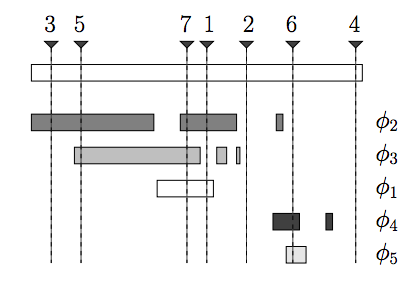
\includegraphics[width=\columnwidth]{brod_paint}}
\caption{\cite{BJP13}  An example feature paintbox spanning the unit interval. Each vertical level below the top rectangle represents a subset of
the unit interval corresponding to a feature. To the right of each subset is
a uniform random label for the feature. If we use the notation of theorem 2.1, the topmost subset is C2 corresponding to feature label $\phi_2$. The
vertical dashed lines represent uniform random draws; i.e., $U′_n$
for index $n$.
The resulting feature allocation of $[7]$ for this realization of the construction is
${{3, 5, 7, 1}, {5, 7}, {7, 1}, {6}, {6}}$. The collection of feature labels for index 7
is $Y_7 = \{\phi_2, \phi_3, \phi_1\}$. The collection of feature labels for index 4 is $Y_4 = \emptyset$. } 
\label{brod_paint}
\end{center}
\vskip -0.2in
\end{figure}


\subsection{Model and Sampler} \label{model}
Here we introduce some notation for the linear gaussian model.  Let $X$ be $N \times D$ data matrix.  Let $Z$ be a $N \times K$ binary matrix drawn from the paintbox.  Let $A$ be a $K \times D$ feature matrix drawn from a normal distribution with variance $\sigma_A^2$.  Let $\epsilon$ be a $N \times D$ matrix of noise with variance $\sigma^2$. Our linear gaussian model takes on the form 
\begin{equation}
X = ZA + \epsilon
\end{equation}
To fully specify our linear gaussian model, we define a prior over the paintbox. The paintbox prior is defined as follows.  Set each conditional $P(F_t = 1|F_{t-1}=f_{t-1},...,F_1=f_1) = \frac
{k}{R}$ for $k \sim \text{DiscreteUniform}(0,R)$ for a "discretization" parameter $R$.  For arbitrary rational approximations, we must take the limit as $R \rightarrow \infty$, which we'll discuss in section \ref{R}.  In this manner, we place a uniform prior on $T$ which completes the description of our model.  The graphical representation is as follows.  

\begin{tikzpicture}[scale=0.2]
\tikzstyle{every node}+=[inner sep=0pt]
\draw [black] (35.7,-10.3) circle (3);
\draw (35.7,-10.3) node {$X$};
\draw [black] (19.4,-24.6) circle (3);
\draw (19.4,-24.6) node {$Z$};
\draw [black] (35.7,-24.6) circle (3);
\draw (35.7,-24.6) node {$A$};
\draw [black] (35.7,-38.2) circle (3);
\draw (35.7,-38.2) node {$\sigma_A$};
\draw [black] (19.4,-38.2) circle (3);
\draw (19.4,-38.2) node {$T$};
\draw [black] (50.7,-24.6) circle (3);
\draw (50.7,-24.6) node {$\sigma$};
\draw [black] (19.4,-51.5) circle (3);
\draw (19.4,-51.5) node {$R$};
\draw [black] (19.4,-35.2) -- (19.4,-27.6);
\fill [black] (19.4,-27.6) -- (18.9,-28.4) -- (19.9,-28.4);
\draw [black] (35.7,-21.6) -- (35.7,-13.3);
\fill [black] (35.7,-13.3) -- (35.2,-14.1) -- (36.2,-14.1);
\draw [black] (35.7,-35.2) -- (35.7,-27.6);
\fill [black] (35.7,-27.6) -- (35.2,-28.4) -- (36.2,-28.4);
\draw [black] (21.66,-22.62) -- (33.44,-12.28);
\fill [black] (33.44,-12.28) -- (32.51,-12.43) -- (33.17,-13.18);
\draw [black] (48.53,-22.53) -- (37.87,-12.37);
\fill [black] (37.87,-12.37) -- (38.11,-13.28) -- (38.8,-12.56);
\draw [black] (19.4,-48.5) -- (19.4,-41.2);
\fill [black] (19.4,-41.2) -- (18.9,-42) -- (19.9,-42);
\end{tikzpicture}

Potentially we can sample $R$ as well but for our purposes $R$ is a gradually increasing parameter and will not be sampled.   We will skip the derivations for $P(X|Z,A,\sigma)$ and $P(A|X,Z,\sigma_A,\sigma)$ for the uncollapsed gibbs sampler, see \cite{DGT09} for details.  The organization of the paper is as follows.  
Section \ref{implementation} provides a thorough description of the sampling algorithms.  First in \ref{nonparametrics} we discuss the nonparametric paintbox which must support dynamically adding and dropping features efficiently whilst preserving the discretization parameter $R$.  Then in \ref{Z} we describe the procedure for sampling the mixing matrix, Z, which is fairly straight-forward.  We then describe sampling the paintbox in \ref{T} which is the computational bottleneck of our inference procedure.  We describe two algorithms, the first is a "standard update" that performs an exponential number $O(2^KR)$ queries of the form $P(Z|T)$.  We introduce an alternative "sparse update" algorithm that performs $O(\min(2^KR,NKR))$ queries of $P(Z|T)$.  The "sparse update" takes advantage of the fact that most of the conditional probabilities in the paintbox need not be updated for $K >> \log N$.  Finally, in \ref{R} we describe the branch-bound procedure that allows us to adaptively increase $R$ without penalizing the runtime.  

In the final section \ref{results} we display the results of the inference on toy data as well as a comparison of the sparse update algorithm to the standard update.  Additionally, we discuss the limitations of our inference procedure and future directions of study.  

If there is any graph you'd like to see, please email me and I can generate them as soon as possible.  As far as previous literature goes, it appears nobody has ever tried to to inference on paintboxes so their will be very few citations going forward.  The code for paintbox inference and generating the graphs is on \href{https://github.com/muherng/cs282/tree/master/code/cs282np-public-master/final}{github}  

\section{Rational Paintboxes} 
% In background, talk about paintboxes generally, here we make specific rational paintboxes 
All exchangeable, consistent, regular feature allocations have an underlying paintbox representation, so we approximate general paintboxes which may contain sequences of countable unions of open intervals with rational intervals for tractable inference.  Our strategy is to set a discretization parameter $R$, such that every conditional probability stored in the paintbox tree is some fraction $\frac{k}{R}$ for integer $k \in [0,R]$.  First, we perform inference on the paintbox for fixed $R$, and then adaptively increase $R$ until we obtain a rational approximation to the underlying paintbox.  In the following section we discuss how we perform efficient inference, how to add and drop features, and how to increase the discretization parameter $R$.       

\section{Efficient Inference with Rational Paintboxes} 
\label{implementation}

% FDV: Paragraph describing the overall inference process 

% FDV: Below might want to be in an algorithm box OR paragraph 
The backbone of the uncollapsed sampler is as follows.   
First we initialize $Z,A,T$. Then we iterate over the following procedures until the sampler is properly mixed.  First we adaptively increase resolution parameter $R$.  Secondly, we add a new feature drawn from base distribution of $A$.  Then we update $Z$ given $X,A,T,\sigma$
\item Update $T$ given $Z,R$
\item Resample $A$ from posterior $P(A|X,Z,\sigma_A,\sigma)$
\item Drop inactive features from $Z,A,$ and $T$
In the next few sections we will focus on steps 3,5,6,7.  

\subsection{Updates for each Variable}
\paragraph{Nonparametrics} \label{nonparametrics}
The nonparametric paintbox requires the tree representation of the paintbox to support adding and dropping features.  Adding features is simply instantiating another layer of $T$ by drawing from the paintbox prior.  On the other hand, dropping features can be achieved by integrating a feature out of the conditional probabilities.  A tricky issue with directly integrating out a feature is that it fails to preserve the discretization parameter $R$.  Instead, we make the entirely reasonable assumption that given another round of updates the probability $$P(F_j = 1|F_{j-1}=f_{j-1},...,F_1=f_1) = 0$$.  Therefore, we update layers $F_k$ for $k \geq j$ by fixing $F_j = 0$ in the conditionals.   
\begin{align*}
P(F_k = f_k|F_{k-1}=f_{k-1},...,F_1=f_1) \leftarrow \\ P(F_{k+1}=f_k|F_k = f_{k-1},...\\...F_{j+1}=f_j,F_j=0, F_{j-1} = f_{j-1},...,F_1=f_1)  
\end{align*} 
Note that the paintbox necessarily doubles in size as it adds a new feature.  So long as we're storing all the conditional probabilities, this exponential blowup is inevitable.  A potential heuristic to workaround these memory demands is to prune the tree for conditionals that are almost never accessed.  Although we don't implement this particular approach in our code, taking advantage of the fact that as the number of active features increases beyond $K >> \log N$  most nodes of the tree are never accessed is a promising direction for taming the memory and run time demands of paintbox inference.  For implications on run time see \ref{T}. For algorithm, see \ref{alg:drop}

\begin{algorithm}[tb]
   \caption{Drop Feature}
   \label{alg:drop}
\begin{algorithmic}
   \STATE {\bfseries Input:} $T,j$ Drop feature $j$ from $T$
   \FOR{$\vec{f} \in \{0,1\}^{j+1}$}
   \IF{$\vec{f}[1] == 0$}
   \STATE $T_{\vec{f}}\text{.parent()} \leftarrow T_{\vec{f}}\text{.parent().parent()}$
   \ENDIF
   \ENDFOR
   \FOR{$\vec{f} \in \{0,1\}^{j}$}
   \STATE $T_{\vec{f}}\text{.parent()} \leftarrow \text{Null}$
   \ENDFOR
   \STATE \textbf{return} T
\end{algorithmic}
\end{algorithm}

% FDV: Make sure that headings for each section match the paragraph above 
\paragraph{Mixing Matrix Update} \label{Z}
Updating $Z$ is fairly straight-forward.  We compute $P(Z|X,A,T,\sigma) \propto P(X|Z,A,\sigma)P(Z|T)$.  The exact update equation for a single row $z \in Z$ is
\begin{equation}
P(z_i|z_{-i},X,A,T,\sigma) \propto P(z|X,A,T,\sigma)P(z|T)
\end{equation}
Where we can compute $P(z|T)$ by querying $T_{z}$.  In the code we store the bottom layer of $T$ as a vector to permit directly indexing for $T_{z}$.  
Since $Z$ has $NK$ entries, we must make $O(NK)$ calls to $P(z|T)$ to sample the mixing matrix.  Since we can directly index for $T_z$, the $Z$ sampling takes a negligible amount of time in comparison to the paintbox updates.  
\subsection{Paintbox Update} \label{T}
Sampling the paintbox is the most computationally expensive step of the inference procedure.  We must re-sample all the conditional probabilities.   In broad strokes, we know that 
\begin{equation}
P(T|Z,R) \propto P(Z|T)P(T|R) = P(Z|T)
\end{equation}
Hence we perform the updates iteratively as follows.  For $j = 1,2,...,K$, for every $\vec{f} = \{f_1,f_2,...,f_j\} \in \{0,1\}^j$, and for every $k \in [R]$ we sample

\begin{aligned}
P(T_{\vec{f}}= \frac{k}{R}|Z,T_{-\vec{f}}) \\ \propto P(Z|T_{-\vec{f}},T_{\vec{f}}= \frac{k}{R})P(T_{\vec{f}} = \frac{k}{R}) \\
\propto P(Z|T_{-\vec{f}},T_{\vec{f}}= \frac{k}{R})
\end{aligned}

Where $T_{-\vec{f}}$ denotes the rest of the tree.  This amounts to $O(2^KR)$ calls to $P(Z|\vec{F} = \vec{f})$ for all $\vec{f} \in \{0,1\}^K$. The exponential dependence in $K$ bottlenecks the inference speed.  Whilst this is by and large inevitable for small $K$, for $K >> \log N$ there are more conditionals to update than there are data points.  It is unnecessary to update conditionals for which there is no corresponding data.  This observation allows us to query $P(Z|\vec{F} = \vec{f})$ a total of $O(\min(2^KR),KNR)$ times.  To better illustrate the difference between the two updates, for $N = 10^6$ data points, and $K=40$ active features, the satndard update calls $P(Z|\vec{F} = \vec{f})$ a trillion times whilst the sparse update will do so only one million times.  The former will never finish running.  In our results, we set up a series of experiments to empirically assess the behavior of this algorithm.  Of course, not every call to $P(Z|\vec{F} = \vec{f})$ takes the same amount of time, and as the paintbox tree increases in size for each additional feature it becomes difficult to pin the run time linearly to $K$.  Nevertheless, the "sparse update" algorithm dramatically decreases the running time of the sampler.  Pseudocode for the standard and sparse updates can be found at \ref{alg:standard} \ref{alg:sparse}


\begin{algorithm}[tb]
   \caption{Standard Update}
   \label{alg:standard}
\begin{algorithmic}
   \STATE {\bfseries Input:} $Z,T$
   \FOR{$j=1$ {\bfseries to} $K$}
   \FOR{$\vec{f} \in \{0,1\}^j$}
   %\State $\text{Roulette} = \emptyset$
   \STATE $\text{Roulette} = \emptyset$
   %\STATE $noChange = false$
   \FOR{$k \in [R]$}
   \STATE $\text{Roulette} $\leftarrow$ \text{Roulette} \cup P(Z|T_{\vec{f}}=\frac{k}{R},T_{-\vec{f}})$
   \ENDFOR
   \STATE \text{Roulette} $\leftarrow \frac{1}{\text{sum}(\text{Roulette})}\text{Roulette}$
   \STATE $T_{\vec{f}} \leftarrow \frac{1}{R}\text{multinomial}(1,\text{Roulette})$
   \ENDFOR
   \ENDFOR
   \STATE \textbf{return} T
\end{algorithmic}
\end{algorithm}

\begin{algorithm}[tb]
   \caption{Sparse Update}
   \label{alg:sparse}
\begin{algorithmic}
   \STATE {\bfseries Input:} $Z,T$
   \IF {$K \leq \log N$}
        \STATE \textbf{return} StandardUpdate(Z,T)
    
   \ENDIF
   \STATE Distinct $\leftarrow$ Set($\{Z_{i,:j} |\forall i \in [N],j\in [K]\}$)
   \FOR{$\vec{f} \in$ Distinct}
   %\State $\text{Roulette} = \emptyset$
   \STATE $\text{Roulette} = \emptyset$
   %\STATE $noChange = false$
   \FOR{$k \in [R]$}
   \STATE $\text{Roulette} $\leftarrow$ \text{Roulette} \cup P(Z|T_{\vec{f}}=\frac{k}{R},T_{-\vec{f}})$
   \ENDFOR
   \STATE \text{Roulette} $\leftarrow \frac{1}{\text{sum}(\text{Roulette})}\text{Roulette}$
   \STATE $T_{\vec{f}} \leftarrow \frac{1}{R}\text{multinomial}(1,\text{Roulette})$
   \ENDFOR
   \STATE \textbf{return} T
\end{algorithmic}
\end{algorithm}

% FDV keep this a separate subsection so it's clear that it's and additional contribution
\subsection{Adaptive Discretization} \label{R}
To approximate rational paintboxes, that is paintboxes of features that are the union of rational intervals, we must adaptively increase the resolution parameter $R$.  Thus far, we've seen that the inference procedure calls $P(Z|T)$ a number of times that varies linearly in $R$.  For $R \rightarrow \infty$ this can become prohibitively expensive.  So we gradually increase $R$, and as we do so we truncate the state space so that we update each conditional probabilities with only a constant number of calls to $P(Z|T)$.  This simple procedure, yields terrific results.  See figures \ref{ll_it} \ref{ll_t} \ref{f_t}


\section{Demonstration on Toy Data}\label{results}

\subsection{Standard vs. Sparse Update}

For our first experiment we compare the standard vs sparse update algorithms for sampling the paintbox.  We graph the per-iteration speed vs the number of active features.  Clearly, sampling the paintbox is slower if it contains more features.  For this experiment, we deliberately set the parameters so that the behaviors of the two algorithms become apparent.  We run the sampler $5$ times for $1000$ iterations on $N = 32$ datapoints with $\sigma = 0.2$ and $\sigma_A = 0.5$.  we choose a small number of data points, and a large amount of noise, and a small $\sigma_A$ to coax the uncollapsed sampler to grab more features. 

As the number of features increases, the standard and sparse algorithms begin to exhibit different run time properties.  Indeed, we chose $N=32$ because we expect the two algorithms to begin diverging at $K = 5$ which is precisely what we observe.  Furthermore, the $O(2^K)$ calls to $P(Z|T)$ is reflected in the exponentially increasing run time of the standard update.

We contrast this to the sparse update algorithm, which runs the standard update up to $K=5$, after which its behavior diverges.  Although, it's hard to say definitively that the subsequent behavior for $K > 5$ varies linearly in $K$, the contrast between the two algorithms is evident.  As we change our experimental parameters to that of our toy experiment, the exponential vs. linear dependence on $K$ of the standard vs. sparse update algorithms becomes less tethered to its empirical run time.  Nevertheless, as we'll see in \ref{sparse_standard} the sparse update still runs much faster than the standard update.  

\begin{figure}[ht]
\vskip 0.2in
\begin{center}
\centerline{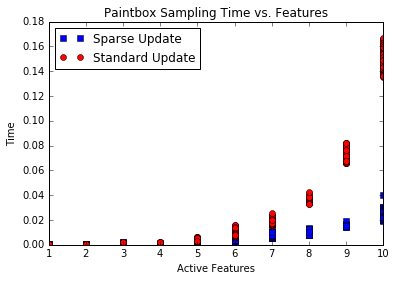
\includegraphics[width=\columnwidth]{alg_scatter}}
\caption{The sparse vs. standard update algorithms for $N = 32$, $\sigma = 0.2$, $\sigma_A = 0.5$.  The two algorithms run the same code up to $K = 5$ after which we would expect exponential increase, $O(2^K)$, in number of calls of $P(Z|T)$ for the standard update vs. a linear increase $O(NK)$ \ for the sparse update.  Here we see that number of calls to $P(Z|T)$ is well correlated with empirical run time}
\label{alg_scatter}
\end{center}
\vskip -0.2in
\end{figure}

For our next experiment, we run the sampler $5$ times for $1000$ iterations on $N = 100$ data points with $\sigma = 0.1$ and $\sigma_A = 0.5$.  These parameters are not quite the same as those used to produce the log likelihood plots.  The reason for this is that we want to coax the algorithm to grab up to 10 features; something it is typically reluctant to do.  

We expect the behaviors of the two update algorithms to diverge at $K = 7$.  Indeed that is what we observe.  Furthermore, the behavior of the standard update appears to be exponential, doubling in iteration time for each additional active feature.  However, the behavior of the sparse update is no longer as tethered to the number of calls to $P(Z|T)$ as it was in the previous experiment.  There are a variety of reasons this may be true.  Firstly, our implementation can be improved, which may make a difference.  Secondly, the size of the paintbox is still doubling for each additional active feature.  The doubling of the memory requirements may begin to tax the empirical run time as the number of features increases.  Finally, calls to $P(Z|T)$ don't all run at the same speed, which is an important assumption in tethering run time to number of calls of a particular function.  Nevertheless, the sparse update clearly outperforms the standard update, a trend that  continues as the number of features increases.                  
\begin{figure}[ht]
\vskip 0.2in
\begin{center}
\centerline{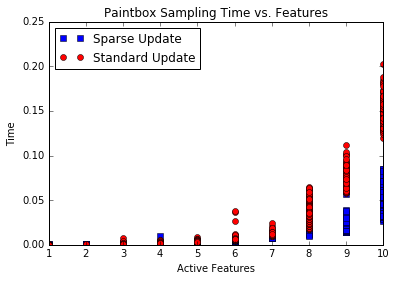
\includegraphics[width=\columnwidth]{sparse_standard}}
\caption{The sparse vs. standard update algorithms for $N = 100$, $\sigma = 0.1$, $\sigma_A = 0.5$.  The two algorithms run the same code up to $K = 6$ after which we would expect exponential increase, $O(2^K)$, in calls to $P(Z|T)$ for the standard update vs. a linear increase $O(NK)$ for the sparse update.  The empirical result is not as crisp as that of \ref{alg_scatter} for reasons delineated in the results.  Nevertheless, the superior run time of the sparse update is exhibited clearly.}
\label{sparse_standard}
\end{center}
\vskip -0.2in
\end{figure} 

\subsection{Comparisons with Indian Buffet Process}

% FDV: Include the paintbox 
We begin with the same four features. Then we correlate and anti-correlate pairs of features as one would expect in a real data set to generate synthetic data.  After running our samplers for both the paintbox and the IBP, we observe 50\% of the dimensions in the held out data, and attempt to recover the rest.  

We generate $2000$ data points, $1000$ of which is used to train, and $1000$ is held out for testing.  The features are arranged in a $6x6$ grid for a total of $36$ dimensions, of which we observe $18$. We display the negative recovered log likelihood for both the paintbox and the uncollapsed IBP in \ref{demo} (smaller is better).  We can see the paintbox is superior to the IBP in settings with correlated and anti-correlated features. 

To better understand the inference, we include a visualization \ref{demo_box} of the paintbox learned from toy data.  The visualization consists of six horizontal bands of light and dark.  Each band corresponds to a feature.  The lightly shaded region corresponds to the presence of a feature, and the dark corresponds to its absence.  Data would then be generated by selecting random draws across the width of the paintbox and selecting the light regions of the features that are intersected.  As discussed, paintboxes are not identifiable so a potentially infinite number of paintboxes can correspond to the same features allocation. 

\begin{figure}[demo]
\vskip 0.2in
\begin{center}
\centerline{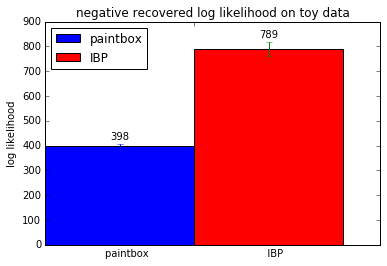
\includegraphics[width=\columnwidth]{demo}}
\caption{We run the sampler on training data, and observe 50\% of held out data.  We graph the negative recovered log likelihood (smaller is better).  The paintbox is superior at reconstructing the held out data from observed dimensions.}
\label{demo}
\end{center}
\vskip -0.2in
\end{figure}

\begin{figure}[demo_box]
\vskip 0.2in
\begin{center}
\textbf{Paintbox Visualization on Toy Data}\par\medskip
\centerline{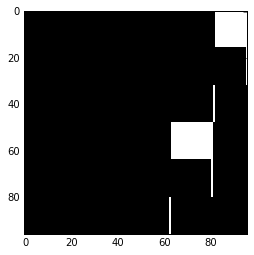
\includegraphics[width=\columnwidth]{demo_box}}
\caption{Visualization of the paintbox learned from synthetic data.  We observe six bands of light and dark.  Each band corresponds to a feature.  Data is generated by generating random draws across the width of the paintbox and selecting features that are light.  Again, many paintboxes correspond to the same feature allocation, but a visualization can aid with intuition for paintbox inference.}
\label{demo_box}
\end{center}
\vskip -0.2in
\end{figure}

\subsection{Adaptive Discretization Demonstration}

For our subsequent experiments we compare the adaptive vs. non-adaptive inference.  As a reminder, the adaptive setting allows us to increase $R$ dynamically without penalizing the run time.  We start with $R = 2$.  Every $100$ iterations we double $R$ and halve its state space to preserve run time so that eventually $R = 1024$.  On the other hand, the non-adaptive setting requires us to fix a value for $R$.  We choose $R = 4$ not by choice, but because larger values of $R$ make it difficult to compare the non-adaptive to the adaptive inference.  We run each of the adaptive and non-adaptive inference algorithms $10$ times for $1000$ iterations for $\sigma = 0.1$ and $\sigma_A = 0.7$.  For the log likelihood comparison see \ref{ll_it} \ref{ll_t}, and for the number of active features over iterations/time see \ref{f_t}.         
\begin{figure}[ht]
\vskip 0.2in
\begin{center}
\centerline{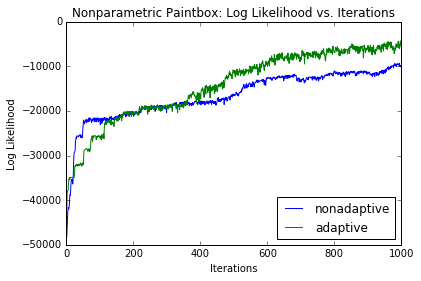
\includegraphics[width=\columnwidth]{ll_it}}
\caption{Adaptive vs Non-adaptive Inference:  The adaptive inference initializes $R = 2$ but scales $R = 1024$ over $1000$ iterations without penalizing the run time by branching and bounding the state space.  The non-adaptive inference sets $R = 4$ and fixes it for $1000$ iterations.  Since the adaptive inference jumps from $R = 2$ to $R = 4$ at iteration $100$ we can see the intersection in the log likelihoods.  The superior performance of the adaptive inference becomes more clear when graphed against time.}
\label{ll_it}
\end{center}
\vskip -0.2in
\end{figure} 
The log likelihood of the adaptive inference initially performs worse than the non-adaptive inference.  The reason is that the adaptive inference initializes $R = 2$ for the first $100$ iterations.  Indeed, we observe that by iteration $100$ the two log likelihoods intersect, and eventually the non-adaptive log likelihood yields to the adaptive one.  Naturally, the adaptive inference samples the paintbox with higher values of $R$, and is therefore a better approximation to general rational paintboxes.            
\begin{figure}[ht]
\vskip 0.2in
\begin{center}
\centerline{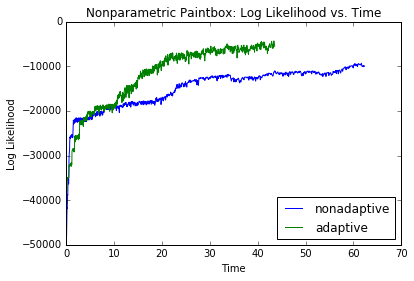
\includegraphics[width=\columnwidth]{ll_t}}
\caption{Adaptive vs. Non-adaptive Inference: Here we plot log likelihood vs. time.  The adaptive inference quickly overtakes the non-adaptive inference, and finishes $1000$ iterations in approximately $45$ seconds}
\label{ll_t}
\end{center}
\vskip -0.2in
\end{figure}
See \ref{ll_t} for the same comparison graphed against time.  We can see that $1000$ iterations of the adaptive inference can run in approximately $45$ seconds whilst the non-adaptive inference takes approximately $65$ seconds.  The reason we set $R=4$ for the non-adaptive case was simply to bring the inference time down to the point where a reasonable comparison of the adaptive and non-adaptive inference could be made.  Here we can see that the adaptive inference outperforms the non-adaptive inference within $5$ seconds owing to the fact that the first $100$ iterations are also the fastest iterations because the number of active features is low.        
\begin{figure}[ht]
\vskip 0.2in
\begin{center}
\centerline{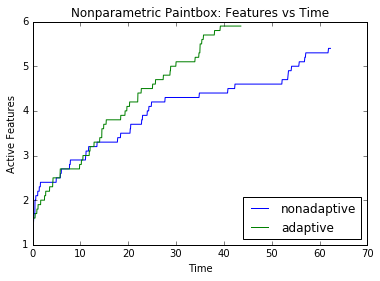
\includegraphics[width=\columnwidth]{f_t}}
\caption{Number of active features over course of inference.  The number of active features is crucial to the run time.  It appears that the adaptive inference learns more features than the non-adaptive inference, but we would need further testing to verify this.}
\label{f_t}
\end{center}
\vskip -0.2in
\end{figure}

The number of active features determines the per iteration run time of the paintbox update which is the computational bottleneck of the inference.  We plot the number of active features sampled over time in both the adaptive and non-adaptive setting.  The adaptive inference appears to learn more features, which may be due to its superior ability to separate correlated features but this is just speculation.  

\begin{figure}[ht]
\vskip 0.2in
\begin{center}
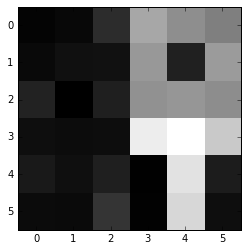
\includegraphics[scale=0.3]{b1}
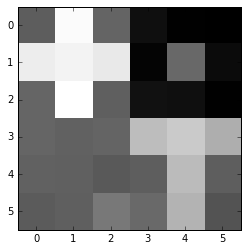
\includegraphics[scale=0.3]{b2}
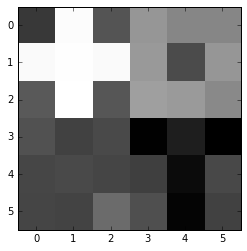
\includegraphics[scale=0.3]{b3}
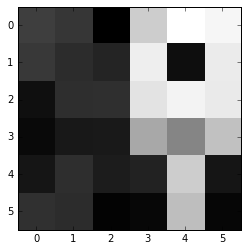
\includegraphics[scale=0.3]{b4}
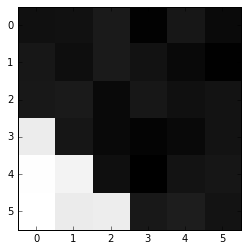
\includegraphics[scale=0.3]{b5}
\caption{Non-adaptive Discretization $R = 4$.  When the discretization is non-adaptive, the run time severely limits the size of $R$.  However, for small values of $R$ the paintbox suffers from the fact that it is a poor approximation to a general rational paintbox and may inadvertently correlate features that are otherwise uncorrelated.}
\label{feature4}
\end{center}
\vskip -0.2in
\end{figure}
In \ref{feature4} we have the features sampled from the posterior mode of $A$ from the non-adaptive inference.  It is clear that at $R=4$ the paintbox mistakenly correlates features, and is sensitive to noise.  The low value of $R$ renders the non-adaptive inference susceptible to a variety of local optima, which the adaptive inference is able to escape from.       

\begin{figure}[ht]
\vskip 0.2in
\begin{center}
\centerline{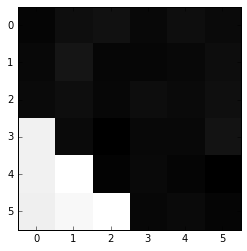
\includegraphics[scale=0.35]{f1}}
\centerline{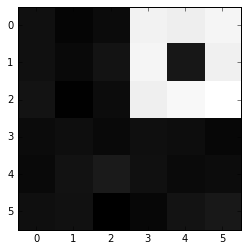
\includegraphics[scale=0.35]{f2}}
\centerline{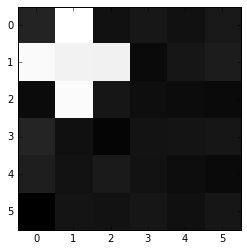
\includegraphics[scale=0.35]{f3}}
\centerline{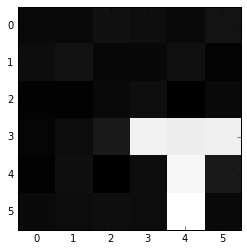
\includegraphics[scale=0.35]{f4}}
\caption{Adaptive Discretization $R = 1024$.  One of the characteristics of paintbox inference is the quality of its feature learning.  The exhaustive nature of its inference is effective at separating features that may be correlated in the data.}
\label{feature1024}
\end{center}
\vskip -0.2in
\end{figure}

See \ref{feature1024} for features learned by the adaptive inference.  In addition to being faster, the adaptive inference can exhaustively learn the conditional probabilities present in the data set, and separate the underlying features from one another.  

\section{Results with Real Data}
\begin{figure}[d1]
\vskip 0.2in
\begin{center}
\centerline{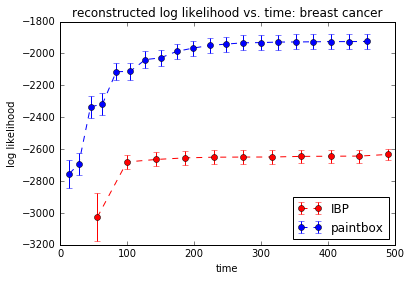
\includegraphics[width=\columnwidth]{d1}}
\caption{breast cancer data set: There are $500$ data points, we held out $100$, and observed $70\%$ of the dimensions of the test data.  The paintbox achieves superior recovered log likelihoods over time.}
\label{d1}
\end{center}
\vskip -0.2in
\end{figure} 

\begin{figure}[d2] 
\vskip 0.2in
\begin{center}
\centerline{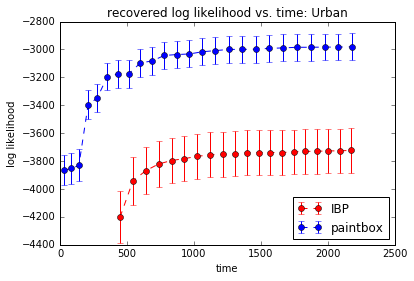
\includegraphics[width=\columnwidth]{d2}}
\caption{Urban data set: We randomly select $1100$ data points, hold out $100$, and observed $70\%$ of the dimensions of the test data.  Paintbox achieves superior recovered log likelihoods over time.}
\label{d2}
\end{center}
\vskip -0.2in
\end{figure} 

\begin{figure}[d3]
\vskip 0.2in
\begin{center}
\centerline{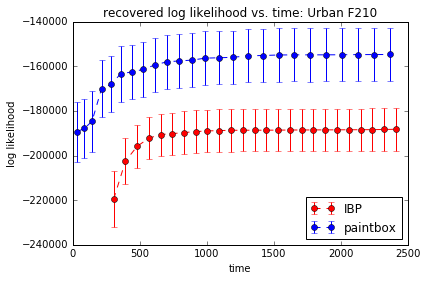
\includegraphics[width=\columnwidth]{d3}}
\caption{Urban F210 data set: We randomly select $1100$ data points, hold out $100$, and observed $70\%$ of the dimensions of the test data.  Paintbox achieves superior recovered log likelihoods over time.}
\label{d3}
\end{center}
\vskip -0.2in
\end{figure} 

% FDV: Put in timing, number of features, test likelihoods, and a qualitative part of at least one data set (show the paintbox and the features).
We run the paintbox inference on real data sets.  We set the noise parameter $\sigma$, and run the uncollapsed IBP for $1000$ iterations.  We employ standard optimization techniques such as initializing the paintbox with output from a simpler model, in this case the IBP, and using random restarts.  The paintbox is initialized with the output of $100$ iterations of the IBP and afterwards we let the paintbox run for $1000$ iterations.      

The breast cancer data set is the smallest with $600$ data points. See figure \ref{d1}  For both Urban data sets, see figures \ref{d2} and \ref{d3}, we randomly selected $1100$ data points allocating $1000$ for training and $100$ for testing.  We randomly observe $70\%$ of the dimensions of the test data from all three data sets.  

Before moving on to qualitative results, it is worth noting that random restarts are critical to the performance of the paintbox.  Sub-optimal outputs from the IBP sampler are rarely improved when fed to the paintbox sampler, whilst higher quality results tend to be improved.  This observation is consistent with our understanding that the paintbox is a more complicated model than the IBP.  Although it is more adept and capturing correlations and anti-correlations, it can be more sensitive to poor initialization.  

\section{Related Work}
% FDV: No inference for paintboxes, but correlated IBP + other stuff like that.
Although there is no work on inference for paintboxes, there has been work in building models that remedy the IBP's assumption that columns of the mixing matrix $Z$ are independent.  The correlated IBP is an example of such a work see \cite{DG12}.  Roughly, the correlated IBP layers another nonparametric process to select "categories" on top of the IBP so as to capture information relating to correlations and anti-correlations.      

\section{Discussion and Conclusion} \label{conclusion}
Just as the graphon is the underlying representation of vertex exchangeable graphs, the feature paintbox is the underlying representation for regular exchangeable feature allocation models \cite{BJP13}.  Consequently, the feature paintbox is a promising candidate for modeling feature allocations in a wider variety of settings than the IBP \cite{gg11}.  To perform inference on paintbox models, we constrain our paintboxes to have only rational conditional probabilities.  Our method of producing rational approximations involves discretizing the paintbox and then adaptively increasing the discretization parameter with a branch and bound approach which allows the discretization to be infinitely fine.  

The primary computational hurdle in our inference procedure is sampling the conditionals in the paintbox which varies exponentially as the number of features increases.  This problem can be partially circumvented with a "sparse" update algorithm that takes advantage of the fact that most of the nodes in the paintbox are never accessed.  In conjunction with the adaptive discretization, sampling the paintbox requires only $O(\min{2^K,NK})$ calls to $P(Z|T)$ as opposed to $O(2^KR)$ calls in the non-adaptive standard update.  We perform a series of experiments empirically verifying the effectiveness of the adaptive inference.  We also perform a series of experiments empirically verifying (to varying degrees) the run time of the sparse update.  

Some difficulties still arise when the number of active features becomes too large, which we suspect is due to the exponentially increasing size of the paintbox tree.  One of the techniques we are trying now is to adaptively prune branches of the paintbox tree that are almost never accessed.  Beyond pruning the paintbox tree, we are tempted to apply our inference procedure to real world data sets to see how it performs.  

In conclusion, we have established that inference on paintbox models is not only  possible but can be done quickly and efficiently despite the "brute-force" nature of its representation.  We have identified the major inference and computational hurdles involved in paintbox inference, and we've developed a few algorithms to overcome these challenges.  Finally, we've identified a few directions for further investigation.     

\bibliography{example_paper}
\bibliographystyle{icml2013}

\end{document} 


% This document was modified from the file originally made available by
% Pat Langley and Andrea Danyluk for ICML-2K. This version was
% created by Lise Getoor and Tobias Scheffer, it was slightly modified  
% from the 2010 version by Thorsten Joachims & Johannes Fuernkranz, 
% slightly modified from the 2009 version by Kiri Wagstaff and 
% Sam Roweis's 2008 version, which is slightly modified from 
% Prasad Tadepalli's 2007 version which is a lightly 
% changed version of the previous year's version by Andrew Moore, 
% which was in turn edited from those of Kristian Kersting and 
% Codrina Lauth. Alex Smola contributed to the algorithmic style files.  
